\chapter{OpenStack Folsom}\label{cap:openstack}

\noindent The current section intends to detail the IaaS Cloud implementation that has been chosen: OpenStack. Initially, a global vision will be given to the reader, to progressively focus on its constituents modules' responsibilities and how they collaborate to maintain the service running.

\section{Global Architecture}\label{sec:arquitecturaglobal}

\noindent Figure \ref{fig:arquitecturaos} shows the three basic operational components of OpenStack Folsom:

\begin{description}
 \item[Functional Core:] OpenStack Compute, OpenStack Quantum and OpenStack Storage (Cinder and Swift).
 \item[Web Management Interface:] OpenStack Horizon.
 \item[Shared Services:] OpenStack Glance, OpenStack Keystone and other related services like a DBMS for persisting meta-data or a messaging queue.
\end{description}

\begin{figure}[tbp]
\begin{center}
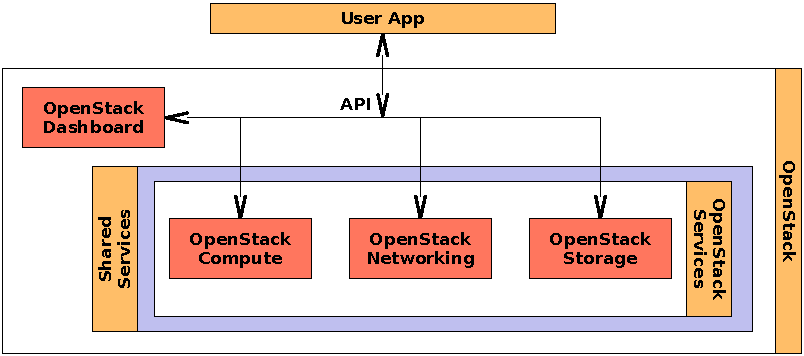
\includegraphics[width=0.9\textwidth]{imagenes/012.pdf}
 \caption{OpenStack Arquitecture}
\label{fig:arquitecturaos}
\end{center}
\end{figure}

The different components have been devised in a shared nothing fashion. This provides the cloud admin the flexibility required to distribute the modules over the cluster as pleased. An example of a particular OpenStack deployment is shown in figure \ref{fig:despliegueos}; OpenStack's own modules are displayed in red, supporting services are shown in violet. What it is missing from the diagram, for clarity, is the asynchronous queue that mediates inter-module communication. Qpid and RabbitMQ are the two queue implementations that are officially documented, being the former the one that we used in our test deployment.

\begin{figure}[tbp]
\begin{center}
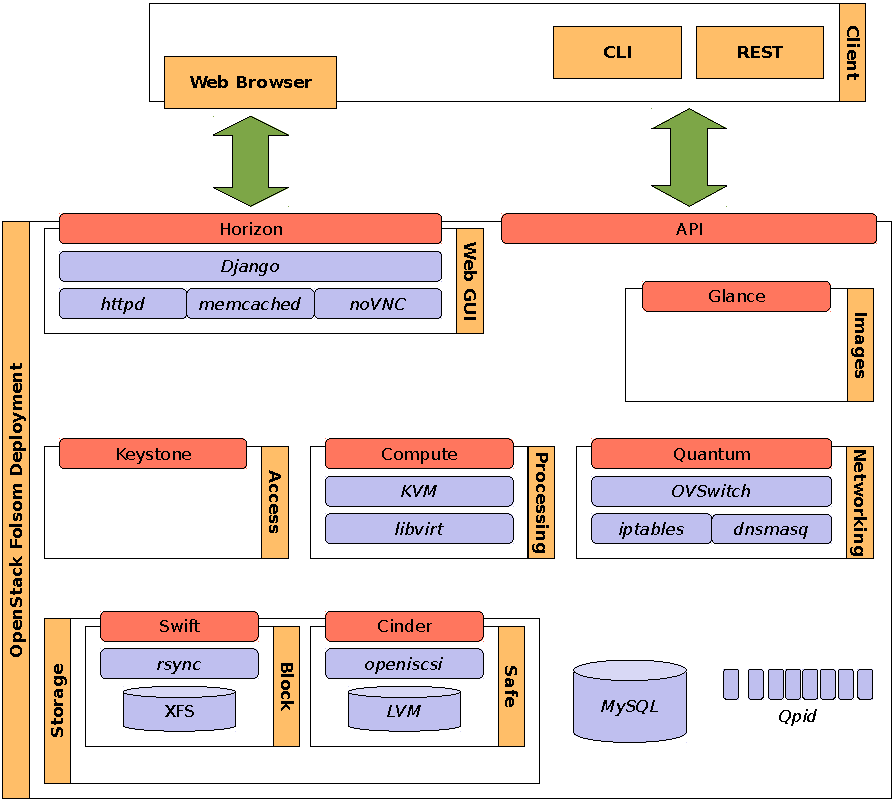
\includegraphics[width=0.99\textwidth]{imagenes/011.pdf}
 \caption{Example of an OpenStack Folsom deployment}
\label{fig:despliegueos}
\end{center}
\end{figure}

\section{Horizon}\label{sec:horizon}

\noident Horizon represents the fundamental window to set up the cloud. As discussed in the previous section, Horizon does not currently --- as of Folsom version --- present a global view of the physical infrastructure, leaving the user in the dark in this respect. Horizon is written in Python on top of \texttt{Django}, the web framework. Django itself relays on a web server like \texttt{httpd} to expose static files, uses a caching mechanism (\texttt{memcached}) to speedup load times and a terminal embedding (\texttt{noVNC}) system to view the output of the virtual graphic card directly on Horizon.

To manage and create instances in the cloud, OpenStack gives the cloud admin the ability to register authorization roles that will let the users consume those services whose role give access to. While the admin is allowed to sign up custom roles, two roles that ship the distribution are the \emph{Cloud Admin} and the \emph{Cloud Member}.

A user granted the admin role will be able to manage:

\begin{description}
 \item[Tenants:] Create, delete, member users, alter quotas, etc.
 \item[Users:] Create, modify or delete.
 \item[OS Images:] List, remove or modify meta-data.
 \item[Instances:] Reset, shutdown, suspend, print log on screen, etc.
 \item[Volumes:] Create, list, attach to an instance, etc.
 \item[Networks:] Create, modify or delete.
\end{description}

A user granted the member role will be able to:

\begin{description}
 \item[Status:] Quota, resources, etc.
 \item[Instances:] create, shutdown, reset, suspend, print log, create image from a running instance (snapshot), etc.
 \item[Volumes:] List, create, modify, attach to an instance, create a volume snapshot, etc.
 \item[Images:] Create, list, delete, modify, etc.
 \item[Networking:] Manage public IPs (floating IPs).
 \item[Security groups:] Create, delete or modify security rules.
 \item[Keypairs:] Create, modify or delete.
\end{description}

\section{Keystone}\label{sec:keystone}

\noindent Keystone is the central security check point and information repository storing information needed to access the cloud installed services. It verifies, before each request, user credentials and authorizations in OpenStack services. Keystone divides this functionality in two parts: on the one hand user control, on the other service catalog.

To deal with users, Keystone assigns them tenants or projects. Users, as discussed above, are granted the membership to a tenant and a service quota they will have to adhere to; they are also restricted to the tenant quota.

To organize the catalog at hand Keystone defines two other concepts within the service catalog: \emph{Services} and \emph{endpoints}. A service in the catalog is a mere abstract description of an exploitable cloud feature by the user. The particular implementation of the service is managed by the set of endpoints associated to it. Said collection contains every piece of information that is required for users to consume the services. Figure \ref{fig:secuenciais} shows a Sequence Diagram portraying the interchanged messages between the different entities taking part to consume a service: \emph{Create a new instance}.

\begin{figure}[tbp]
\begin{center}
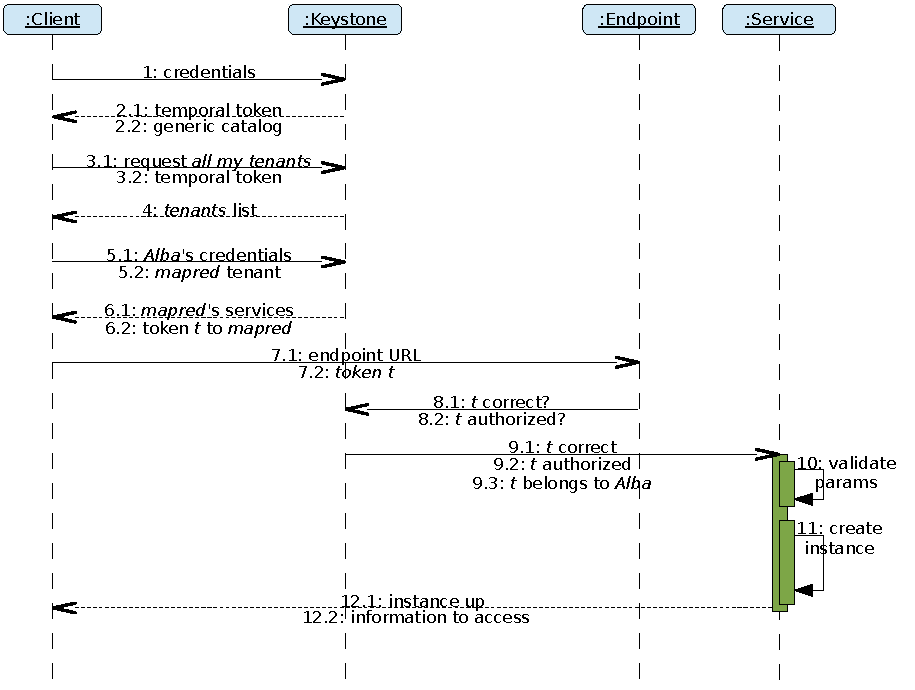
\includegraphics[width=0.99\textwidth]{imagenes/013.pdf}
 \caption{Sequence Diagram --- create instance}
\label{fig:secuenciais}
\end{center}
\end{figure}

Stemming from the fact that Horizon exposes only a part of OpenStack functionality, Keystone includes a CLI tool to interact with the REST service in charge of administrative operations to help dealing with administrative operations. Issuing certain commands to Keystone through a terminal requires the knowledge of the admin token, which has to be conveniently secured, or the login credentials of a user with the admin role. Lastly, it should be noted that Keystone uses a data base to store user access credentials and the service catalog meta-data.

\section{Quantum}\label{sec:quantum}

\noindent Starting in Folsom, Quantum is the module to manage virtual networking. It was introduced to separate the networking part from the computing part, held together in \texttt{Compute} module. Certainly, the fact that it had been refactored out demonstrates OpenStack's evolving model toward a more coherent less coupled functional allocation; and as it is independent, it could be configured in a dedicated node.

To bring virtual networking into existence Quantum banks on external plug-ins. Two of those plug-ins whose usage is covered in the official Quantum administrator manual (\cite{quantumadminfolsom}) are \texttt{OpenVSwitch} and \texttt{LinuxBridge}. Additionally, Quantum relies on iptables to configure routing rules and firewall, \texttt{dnsmasq} for the \emph{DNS}, the \emph{DHCP} and the \emph{NAT}.

Figure \ref{fig:desplieguequantum} pictures a topology example of a virtual network. On it, \emph{30.0.0.X} represent public IPs and \emph{10.0.X.Y} private. This virtual network assigns a virtual router to each tenant but more could be added with ease. Private IP overlapping over different networks is possible as expected (\emph{10.0.0.2}). The routers public IPs --- they could be assigned more external interfaces --- must be taken from the external network (\emph{30.0.0.0}).

\begin{figure}[tbh]
\begin{center}
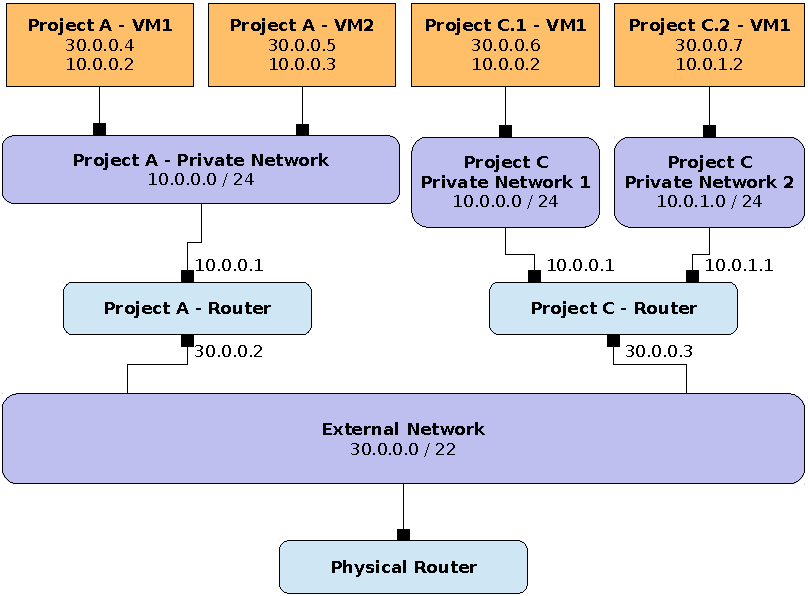
\includegraphics[width=0.9\textwidth]{imagenes/014.pdf}
 \caption{Virtual network deployment with Quantum}
\label{fig:desplieguequantum}
\end{center}
\end{figure}

\section{Compute}\label{sec:compute}

\noindent Compute is the central module. Its duty entails orchestrating the global workings in the cloud, delegating each particular function to the service on charge. In the end, Compute will let a logged user start virtual instances, which will draw their VCPU, VRAM and VHDD from the physical cluster. Yet required, Compute does not contain a virtualization package. The approach is to delegate infrastructure provision to a hypervisor found typically, but not restricted to, in the same node. To expose this on-demand computational service, Compute implements a REST API so that users can control their instances' life cycle directly from a REST client (like the CLI tools that accompany Compute).

To create effectively create an instance, Compute will communicate with other modules within the cloud to orchestrate the execution and, finally, it will pass the request to the most suitable cluster node's hypervisor --- most suitable according to the cloud-defined rule set --- that will bring up the VM. Some of the supporting services are described bellow.

\begin{description}
 \item[Keystone:] Matches supplied vs. stored credentials, clearing or refusing requests.
 \item[Glance:] Finds the OS image that should be run.
 \item[Quantum:] Provides private and public IPs and checks network flow to/from the instance.
 \item[Cinder:] Drives block storage and so it is in charge of exposing \emph{hot-plugged} volumes into the instance.
 \item[Qpid:] Enables message passing among the different modules.
\end{description}

It has been said throughout the text that if there is a something aligning the differing IaaS implementations is their flexibility. Users' computational needs vary with time, so it seems reasonable to think they will expect their virtual services to adapt to them. Hypervisors have fulfilled this behavior since their design, making them ideal matches to help serve infrastructure as a service. OpenStack nomenclature --- inspired by AWS' --- calls each possible particular VM specification a \emph{flavor}.

Se ha venido diciendo a lo largo del texto que si algo alinea a los distintos cloud es su flexibilidad. Puesto que las necesidades computacionales de los usuarios var\'ian en funci\'on del tiempo, es necesario que, dentro de unos l\'imites, se les permita concretar las caracter\'isticas t\'ecnicas de las m\'aquinas virtuales. En OpenStack cada posible configuraci\'on instanciable, esto es, cada realizaci\'on concreta de la cantidad de recursos que temporalmente se expropian del anfitri\'on, se denomina \emph{flavor} ---siguiendo la nomenclatura de los AWS. De manera que se va a otorgar la posibilidad de que los usuarios autorizados puedan crear sus propios \emph{sabores} computacionales, definiendo el tama\~no del disco, el n\'umero de VCPUs, etc., sin ninguna dificultad, a trav\'es de Horizon.


\section{Glance}\label{sec:glance}
\noindent Glance es el servicio de hospedaje de im\'agenes para OpenStack. Se pueden configurar m\'ultiples backends de datos para guardarlas como: Swift, Amazon S3, el sistema de ficheros local o una ubicaci\'on HTTP; lo que mantiene el nivel de flexibilidad a la par con los dem\'as m\'odulos. Glance se vale de Keystone para manejar el acceso y la seguridad de las im\'agenes y se comunica con Compute para ponerlas en ejecuci\'on bajo demanda.
Ofrece soporte a una buena variedad de clases de im\'agenes y formatos de su contenedor; pero este hecho es meramente informativo para el cloud, ya que la capacidad o incapacidad de arrancar una instancia est\'a vinculada al hipervisor desplegado y no a Glance. Tambi\'en est\'a presente la habilidad de asociar metadatos a las im\'agenes en forma de pares \texttt{(clave, valor)}. Esta metainformaci\'on se utiliza para diferenciar distintas im\'agenes o para configurar el \emph{direct kernel boot} necesario para redimensionar el volumen ra\'iz al arrancar las im\'agenes en distintos sabores.


\section{Almacenamiento}\label{sec:almacenamiento}
\noindent OpenStack otorga tres opciones a la hora de elegir el tipo de almacenamiento:
\begin{description}
 \item[Vol\'atil:] las dimensiones del disco r\'igido sobre el que se dispone la ra\'iz del \'arbol de ficheros se fijan, en el momento de arrancar la m\'aquina virtual, a las marcadas por el sabor elegido. Los archivos contenidos en \'el son aquellos que aparecen en la definici\'on de la imagen del sistema almacenada en Glance. Las alteraciones de este sistema de ficheros no persisten entre ejecuciones de las instancias. Al ordenar la finalizaci\'on de la ejecuci\'on de un servidor virtual, se destruye el fichero temporal que reflejaba las modificaciones del usuario a dicho sistema de ficheros en esa ejecuci\'on concreta.
 \item[Persistente:] vali\'endose de vol\'umenes de almacenamiento gestionados por Cinder con ayuda de \emph{LVM} (\emph{Logical Volume Manager}), OpenStack otorga la posibilidad de enganchar a las instancias, en caliente, vol\'umenes l\'ogicos de tama\~nos indeterminados y creados bajo demanda. Con este tipo de salvaguarda, se garantiza que la informaci\'on no se pierde al terminar la sesi\'on de ejecuci\'on. Sin embargo, este mecanismo de almacenamiento tiene una importante limitaci\'on y es que no es posible enganchar un mismo volumen l\'ogico a dos instancias al mismo tiempo. La alta disponibilidad o la seguridad de la informaci\'on ante fallo no est\'an implementadas directamente, ya que los datos van a residir en un \'unico punto. Podr\'ian superarse estas limitaciones definiendo alguna pol\'itica de copia de seguridad o alguna cofiguraci\'on \emph{RAID} (\emph{Redundant Array of Idependent Disks}) sobre los vol\'umenes ---no recomendable porque OpenStack cuenta con un m\'odulo a tal fin (Swift).
 \item[Seguro:] OpenStack Swift es el m\'odulo que permite la gesti\'on autom\'atica del almacenamiento distribuido de forma segura y permitiendo despliegues para alta disponibilidad. Utiliza la replicaci\'on controlada para establecer el marco de seguridad y la alta disponibilidad, combatiendo as\'i los problemas derivados de la fragilidad inherente a los discos duros. Swift se escuda en \texttt{rsync} para sincronizar las r\'eplicas sobre particiones \emph{XFS}.
\end{description}


\subsection{Cinder}\label{subsec:cinder}
\noindent Cinder es el m\'odulo de OpenStack que maneja los dispositivos virtuales de almacenamiento en bloque; de funcionalidad similar a la del \emph{EBS} (\emph{Elastic Block Storage}) de Amazon. Cinder utiliza una implementaci\'on de \emph{iSCSI} (\texttt{open-iscsi}) y LVM para Linux para gestionar las operaciones sobre los vol\'umenes. La creaci\'on, el enganche y desacople y el borrado de los bloques de almacenamiento persistente se maneja desde Horizon directamente.\newline

Estos bloques virtuales de persistencia se gestionan como vol\'umenes l\'ogicos pertenecientes a un grupo de vol\'umenes controlado por Cinder. Cinder no pretende crear un medio compartido como \emph{NFS} (\emph{Network File System}), o alguna soluci\'on \emph{SAN} (\emph{Storage Area Network}) o \emph{NAS} (\emph{Network Attached Storage}) para las instancias, ya que no es posible compartir un mismo vo\-lu\-men l\'ogico con m\'as de una m\'aquina virtual en un mismo instante. Una opci\'on interesante, que permite Cinder para facilitar ciertos despligues virtuales heterog\'eneos, es configurar las instancias para que arranquen desde un volumen creado por Cinder.


\subsection{Swift}\label{subsec:swift}
\noindent Al igual que suced\'ia con Cinder, Swift tampoco se enmarca en la idea tradicional de almacenamiento compartido en red, ni debe compararse con el anterior; Cinder y Swift cubren demandas diferentes. Se dice que Swift es ``\textit{un sistema escalable de almacenamiento de objetos, donde los usuarios registrados controlan sus compartimentos de datos o contenedores, subiendo, descargando o borrando ficheros a su antojo}'' \cite{osswift}. Funcionalmente Swift equivale al S3 de Amazon y al \texttt{Walrus} de Eucalyptus, siendo posible con\-fi\-gu\-rar un API REST compatible, parcialmente por el momento (enero 2013), con la sintaxis del primero. Una caracter\'istica fundamental para Swift es la replicaci\'on controlada.


\subsubsection{Replicaci\'on}\label{subsubsec:replicacion}
\noindent La escalabilidad, la tolerancia a fallo, la alta disponibilidad, la seguridad, el balanceo de almacenamiento y el control de carga son algunos de los rasgos que definen a Swift. La alta disponibilidad y la tolerancia a fallo se implementan usando la replicaci\'on. La replicaci\'on es un mecanismo a trav\'es del cual un sistema distribuido mantiene copias o \emph{r\'eplicas} en puntos diferentes de su despliegue, para mejorar sus prestaciones o limitar el alcalce de los fallos, entre otros.\newline

En Swift, los procesos de replicaci\'on de cada \emph{Servidor de Objetos}, que es un nodo cualquiera del cl\'uster con Swift en funcionamiento, van a comparar, peri\'odicamente, sus copias locales con cada copia remota para verificar su grado de actualizaci\'on. Cotejar estas r\'eplicas es un proceso tan costoso computacionalmente como habitual en sistemas de almacenamiento distribuido, por eso Swift se vale de estructuras como las \emph{listas Hash} o las \emph{marcas de agua} para acelerar las comparaciones. Rsync o HTTP gestionan la trans\-fe\-ren\-cia de las copias en funci\'on del tipo de objeto a replicar. La transparencia de replicaci\'on es uno de los pilares que soportan la escalabilidad de Swift. Cuando se a\~nade un nuevo nodo al espacio de almacenamiento de Swift, la redistribuci\'on de las copias es autom\'atica y, desde el momento en que \'este sea sincronizado, podr\'a responder a peticiones de datos de los usuarios.

\subsubsection{Updaters y Auditors}\label{subsubsec:otroscompswift}
\noindent Otros componentes interesantes, que completan el c\'irculo funcional descrito para Swift, son los \emph{Updaters} y los \emph{Auditors}. Los primeros act\'uan cuando se produce un error de sincronizaci\'on entre copias o cuando la carga computacional de un Servidor de Objetos es lo suficientemente alta como para que no pueda satisfacer una operaci\'on. Sucede entonces que la ejecuci\'on de esa operaci\'on se difiere; se a\~nade a una cola de actualizaci\'on que el Updater va procesando para restablecer la sincronizaci\'on. Los Auditors escanean continuamente el sistema de ficheros en busca de fallos de integridad en objetos, contenedores o cuentas de usuario, tal que, si encontrasen incoherencias, pondr\'ian en cuarentena a la entidad y pedir\'ian que se estableciese una nueva r\'eplica.
